\XtoCBlock{AdaptiveNotch}
\label{block:AdaptiveNotch}
\begin{figure}[H]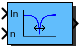
\includegraphics{AdaptiveNotch}\end{figure} 

\begin{XtoCtabular}{Inports}
In & Input signal\tabularnewline
\hline
n & Speed input = notch frequency\tabularnewline
\hline
\end{XtoCtabular}


\begin{XtoCtabular}{Outports}
Out & Filtered output signal\tabularnewline
\hline
\end{XtoCtabular}

\begin{XtoCMaskParamTabular}{Mask Parameters}
\rowcolor[gray]{0.8}\textbf{Name} & \textbf{ID} & \textbf{Description}\tabularnewline\hline
Q & 1 & Q-Factor of the notch filter\tabularnewline
\hline
n\_thresh & 2 & Speed threshold for activating the filter\tabularnewline
\hline
n\_max & 3 & Maximum revolutions per minute

(Not used in floating point implementations)\tabularnewline
\hline
p & 4 & Number of pole pairs\tabularnewline
\hline
ts\_fact & 5 & Multiplication factor of base sampling time (in integer format)\tabularnewline
\hline
method & 6 & Discretization method\tabularnewline
\hline
\end{XtoCMaskParamTabular}

\subsubsection*{Description:}
Notch filter with variable notch frequency

% include optional documentation file
\InputIfFileExists{\XcHomePath/Library/Filter/Doc/AdaptiveNotch_Info.tex}{\vspace{1ex}}{}

\subsubsection*{Implementations:}
\begin{tabular}{l l}
\textbf{FiP16} & 16 Bit Fixed Point Implementation\tabularnewline
\textbf{FiP32} & 32 Bit Fixed Point Implementation\tabularnewline
\textbf{Float32} & 32 Bit Floating Point Implementation\tabularnewline
\textbf{Float64} & 64 Bit Floating Point Implementation\tabularnewline
\end{tabular}

\XtoCImplementation{FiP16}
\nopagebreak[0]

16 Bit Fixed Point Implementation

\begin{XtoCtabular}{Inports Data Type}
In & int16\tabularnewline
\hline
n & int16\tabularnewline
\hline
\end{XtoCtabular}

\begin{XtoCtabular}{Outports Data Type}
Out & int16\tabularnewline
\hline
\end{XtoCtabular}

\ifdefined \AddTestReports
\InputIfFileExists{\XcHomePath/Library/Filter/Doc/Test-Results/Test_AdaptiveNotch_FiP16.tex}{}{}
\fi
\XtoCImplementation{FiP32}
\nopagebreak[0]

32 Bit Fixed Point Implementation

\begin{XtoCtabular}{Inports Data Type}
In & int32\tabularnewline
\hline
n & int32\tabularnewline
\hline
\end{XtoCtabular}

\begin{XtoCtabular}{Outports Data Type}
Out & int32\tabularnewline
\hline
\end{XtoCtabular}

\ifdefined \AddTestReports
\InputIfFileExists{\XcHomePath/Library/Filter/Doc/Test-Results/Test_AdaptiveNotch_FiP32.tex}{}{}
\fi
\XtoCImplementation{Float32}
\nopagebreak[0]

32 Bit Floating Point Implementation

\begin{XtoCtabular}{Inports Data Type}
In & float32\tabularnewline
\hline
n & float32\tabularnewline
\hline
\end{XtoCtabular}

\begin{XtoCtabular}{Outports Data Type}
Out & float32\tabularnewline
\hline
\end{XtoCtabular}

\ifdefined \AddTestReports
\InputIfFileExists{\XcHomePath/Library/Filter/Doc/Test-Results/Test_AdaptiveNotch_Float32.tex}{}{}
\fi
\XtoCImplementation{Float64}
\nopagebreak[0]

64 Bit Floating Point Implementation

\begin{XtoCtabular}{Inports Data Type}
In & float64\tabularnewline
\hline
n & float64\tabularnewline
\hline
\end{XtoCtabular}

\begin{XtoCtabular}{Outports Data Type}
Out & float64\tabularnewline
\hline
\end{XtoCtabular}

\ifdefined \AddTestReports
\InputIfFileExists{\XcHomePath/Library/Filter/Doc/Test-Results/Test_AdaptiveNotch_Float64.tex}{}{}
\fi
